\documentclass[tikz,border=2pt]{standalone}
\usepackage[T1]{fontenc}
\usepackage{helvet,amsmath,amssymb,fix-cm}
\renewcommand{\familydefault}{\sfdefault}
\usetikzlibrary{arrows.meta,calc,positioning,fit,backgrounds,decorations.pathreplacing,shapes.geometric}
\definecolor{ink}{HTML}{243343}
\definecolor{physical}{HTML}{3478A3}
\definecolor{semantic}{HTML}{B27C26}
\definecolor{feasible}{HTML}{248679}
\definecolor{decode}{HTML}{75609D}
\definecolor{fault}{HTML}{BA5554}
\definecolor{muted}{HTML}{6F7D88}
\tikzset{
  every node/.style={font=\fontsize{9}{10.8}\selectfont,text=ink},
  edge/.style={-{Stealth[length=1.8mm,width=1.25mm]},line width=.6pt,draw=ink},
  param/.style={-{Stealth[length=1.7mm]},line width=.6pt,draw=decode,dashed},
  link/.style={line width=.8pt,draw=physical},
  reject/.style={line width=.7pt,draw=fault,dashed},
  panel/.style={rounded corners=2pt,draw=muted!45,line width=.45pt,fill=white},
  box/.style={rounded corners=2pt,draw=physical!70,line width=.55pt,fill=physical!6,align=center,inner sep=3pt},
  sem/.style={box,draw=semantic!70,fill=semantic!8},
  gate/.style={box,draw=feasible!70,fill=feasible!7},
  dec/.style={box,draw=decode!70,fill=decode!7},
  tinylabel/.style={font=\fontsize{8}{9.4}\selectfont},
  smalllabel/.style={font=\fontsize{8.5}{10}\selectfont},
  heading/.style={font=\bfseries\fontsize{10}{11.5}\selectfont,anchor=north west},
  dot/.style={circle,minimum size=.43cm,inner sep=0pt,draw=physical,fill=white,line width=.8pt,font=\bfseries\fontsize{9}{10}\selectfont},
  receiver/.pic={\draw[draw=physical,line width=.8pt] (0,0)--(0,.58) (-.17,0)--(.17,0) (-.15,.39)--(0,.58)--(.15,.39);
    \draw[draw=physical!70,line width=.55pt] (-.2,.56) arc[start angle=160,end angle=200,radius=.23];
    \draw[draw=physical!70,line width=.55pt] (.2,.40) arc[start angle=-20,end angle=20,radius=.23];},
}
\begin{document}
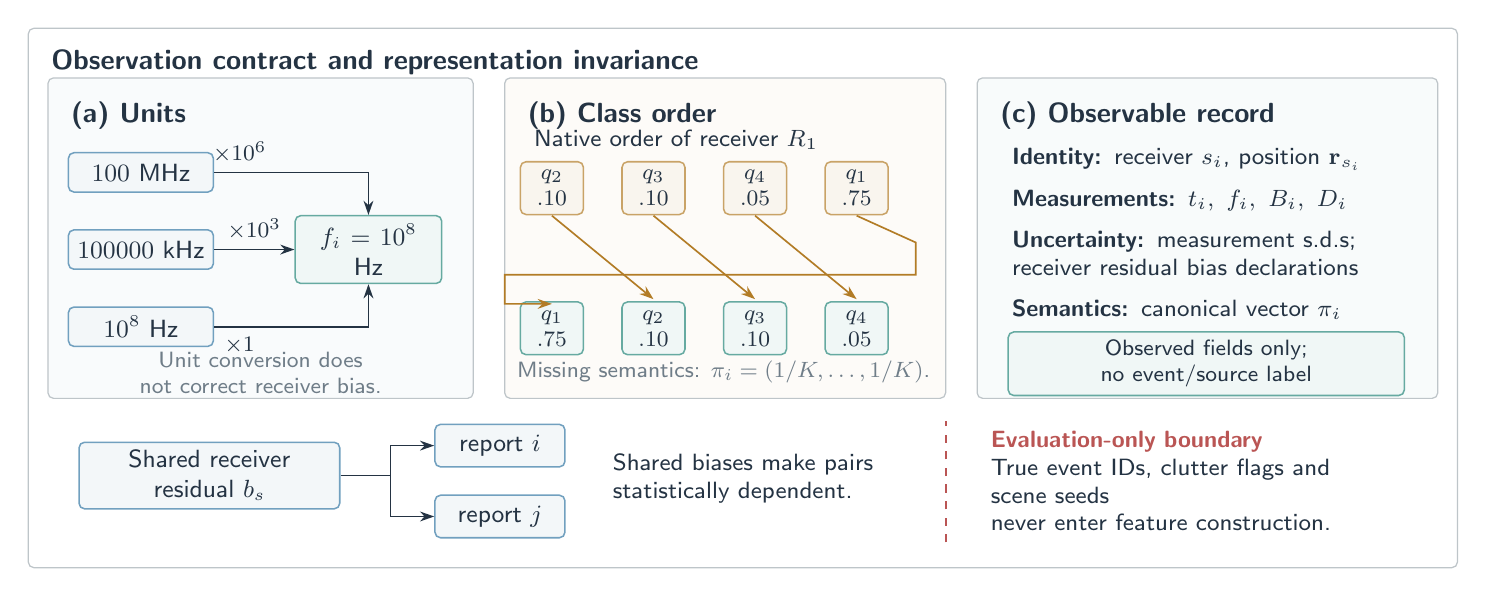
\begin{tikzpicture}[x=1cm,y=1cm]
\draw[panel] (0,0) rectangle ++(18.15,6.85);
\node[heading] at (0.17,6.699999999999999) {Observation contract and representation invariance};

\draw[panel,fill=physical!3] (.25,2.15) rectangle (5.65,6.22);
\draw[panel,fill=semantic!3] (6.05,2.15) rectangle (11.65,6.22);
\draw[panel,fill=feasible!3] (12.05,2.15) rectangle (17.90,6.22);
\node[heading] at (.42,6.04) {(a) Units};
\node[heading] at (6.22,6.04) {(b) Class order};
\node[heading] at (12.22,6.04) {(c) Observable record};
\node[box,text width=1.63cm,minimum height=.5cm] (mhz) at (1.43,5.02) {$100$ MHz};
\node[box,text width=1.63cm,minimum height=.5cm] (khz) at (1.43,4.04) {$100000$ kHz};
\node[box,text width=1.63cm,minimum height=.5cm] (hz) at (1.43,3.06) {$10^8$ Hz};
\node[gate,text width=1.65cm,minimum height=.65cm] (canon) at (4.32,4.04) {$f_i=10^8$ Hz};
\draw[edge] (mhz.east)--node[above,tinylabel] {$\times10^6$} (3.01,5.02)-|(canon.north);
\draw[edge] (khz.east)--node[above,tinylabel] {$\times10^3$} (canon.west);
\draw[edge] (hz.east)--node[below,tinylabel] {$\times1$} (3.01,3.06)-|(canon.south);
\node[tinylabel,text width=4.8cm,align=center,text=muted] at (2.95,2.48) {Unit conversion does not correct receiver bias.};

\node[smalllabel,anchor=west] at (6.3,5.43) {Native order of receiver $R_1$};
\foreach \xx/\lab/\val in {6.65/2/.10,7.94/3/.10,9.23/4/.05,10.52/1/.75}{
  \node[sem,minimum width=.80cm,minimum height=.67cm,tinylabel] at (\xx,4.82) {$q_{\lab}$\\$\val$};}
\foreach \xx/\lab/\val in {6.65/1/.75,7.94/2/.10,9.23/3/.10,10.52/4/.05}{
  \node[gate,minimum width=.80cm,minimum height=.67cm,tinylabel] at (\xx,3.04) {$q_{\lab}$\\$\val$};}
\draw[edge,semantic] (6.65,4.47)--(7.94,3.41);
\draw[edge,semantic] (7.94,4.47)--(9.23,3.41);
\draw[edge,semantic] (9.23,4.47)--(10.52,3.41);
\draw[edge,semantic] (10.52,4.47)--(11.27,4.13)--(11.27,3.72)--(6.05,3.72)--(6.05,3.35)--(6.65,3.35);
% Class-order mapping is shown by edges; no annotation is drawn on top of them.
\node[tinylabel,text=muted] at (8.83,2.49) {Missing semantics: $\pi_i=(1/K,\ldots,1/K)$.};

\node[anchor=north west,align=left,text width=5.15cm,smalllabel] at (12.37,5.45) {
\textbf{Identity:} receiver $s_i$, position $\mathbf r_{s_i}$\\[5pt]
\textbf{Measurements:} $t_i,\ f_i,\ B_i,\ D_i$\\[5pt]
\textbf{Uncertainty:} measurement s.d.s;\\receiver residual bias declarations\\[5pt]
\textbf{Semantics:} canonical vector $\pi_i$};
\node[gate,text width=4.82cm,minimum height=.42cm,tinylabel] at (14.96,2.59) {Observed fields only; no event/source label};

\node[box,text width=3.1cm,minimum height=.77cm] (shared) at (2.3,1.17) {Shared receiver\\residual $b_s$};
\node[box,text width=1.44cm,minimum height=.54cm] (oa) at (5.99,1.55) {report $i$};
\node[box,text width=1.44cm,minimum height=.54cm] (ob) at (5.99,.65) {report $j$};
\draw[edge] (shared.east)--(4.60,1.17)|-(oa.west);
\draw[edge] (4.60,1.17)|-(ob.west);
\node[smalllabel,align=left,anchor=west,text width=3.55cm] at (7.3,1.13)
 {Shared biases make pairs\\statistically dependent.};
\draw[draw=fault,dashed,line width=.7pt] (11.66,.32)--(11.66,1.86);
\node[anchor=west,align=left,text width=5.1cm,smalllabel] at (12.1,1.1)
 {\textcolor{fault}{\textbf{Evaluation-only boundary}}\\True event IDs, clutter flags and scene seeds\\never enter feature construction.};
\end{tikzpicture}
\end{document}
